

\preClass{Integral Calculus Review}

\begin{problem}
\item Find the solutions to the following integrals. In each case
  solve for $y$ in terms of $t$. (Do not forget the ``$+C$''
  associated with each indefinite integral!)
  \begin{subproblem}
    \item $y = \int \cos(3t) ~ dt$

      \iftoggle{solutions}{%
        \begin{eqnarray*}
          y & = & \frac{1}{3} \sin(3t) + C.
        \end{eqnarray*}
      }

      \vfill
    \item $y = \int t^2 + e^{5t} ~ dt$

      \iftoggle{solutions}{%
        \begin{eqnarray*}
          y & = & \frac{1}{3} t^3 + \frac{1}{5} e^{5t} + C.
        \end{eqnarray*}        
      }

      \vfill
    \item $t = \int \frac{1}{y} ~ dy$

      \iftoggle{solutions}{%
        \begin{eqnarray*}
          t & = & \ln(y) + C, \\
          \ln(y) & = & t-C, \\
          y & = & e^{t-c}, \\
          y & = & e^t e^{-c}, \\
          y & = & k e^t.
        \end{eqnarray*}
      }

      \vfill
    \item $t = \int y^2 ~ dy$

      \iftoggle{solutions}{%
        \begin{eqnarray*}
          t & = & \frac{1}{3} y^3 + C, \\
          \frac{1}{3} y^3 & = & t - C, \\
          y^3 & = & 3(t - C), \\
          y & = & \sqrt[3]{3(t-C)}.
        \end{eqnarray*}
      }

      \vfill
  \end{subproblem}  
\end{problem}


\actTitle{Basic Integrals and Slope Fields}
\begin{problem}
\item Find the solutions to the following integrals. In each case
  solve for $y$ in terms of $t$. (Do not forget the ``$+C$''
  associated with each indefinite integral!)
  \begin{subproblem}
    \item $y = \int t\cos(3t) ~ dt$

      \iftoggle{solutions}{%

        \begin{eqnarray*}
          y & = & \int t\cos(3t) ~ dt, \\
            & = & \frac{1}{3} t \sin(3t) + \frac{1}{9} \cos(3t) + C.
        \end{eqnarray*}
        
      }

      \vfill
    \item $y = \int t e^{5t} ~ dt$

      \iftoggle{solutions}{%

        \begin{eqnarray*}
          y & = & \int t e^{5t} ~ dt, \\
            & = & \frac{1}{5} t e^{5t} - \frac{1}{25} e^{5t} + C.
        \end{eqnarray*}
        
      }

      \vfill
    \item $y = \int t^2 \ln(t) ~ dt$

      \iftoggle{solutions}{%
        
        \begin{eqnarray*}
          y & = & \int t^2 \ln(t) ~ dt, \\
            & = & \frac{1}{3} t^3 \ln(t) - \frac{1}{9} t^3 + C.
        \end{eqnarray*}

      }

      \vfill
    \item $t = \int \frac{\ln(y)}{y} ~ dy$

      \iftoggle{solutions}{%

        \begin{eqnarray*}
          t & = & \int \frac{\ln(y)}{y} ~ dy, \\
            & = & \half \lp \ln(y) \rp^2 + C, \\
          \pm \sqrt{2(t-C)} & = & \ln(y), \\
          y & = & e^{\pm \sqrt{2(t-C)}}.
        \end{eqnarray*}
        
      }

      \vfill
  \end{subproblem}

\clearpage

\item For each slope field make sketches for different solutions for
  each of the following initial conditions:
  \begin{eqnarray*}
    y(0) & = & 3, \\
    y(0) & = & 1, \\
    y(0) & = & 0, \\
    y(0) & = & -1, \\
    y(0) & = & -3.
  \end{eqnarray*}
  For each slope field state the general behavior and state the long
  term solutions if they exist.

  \begin{subproblem}
    \item 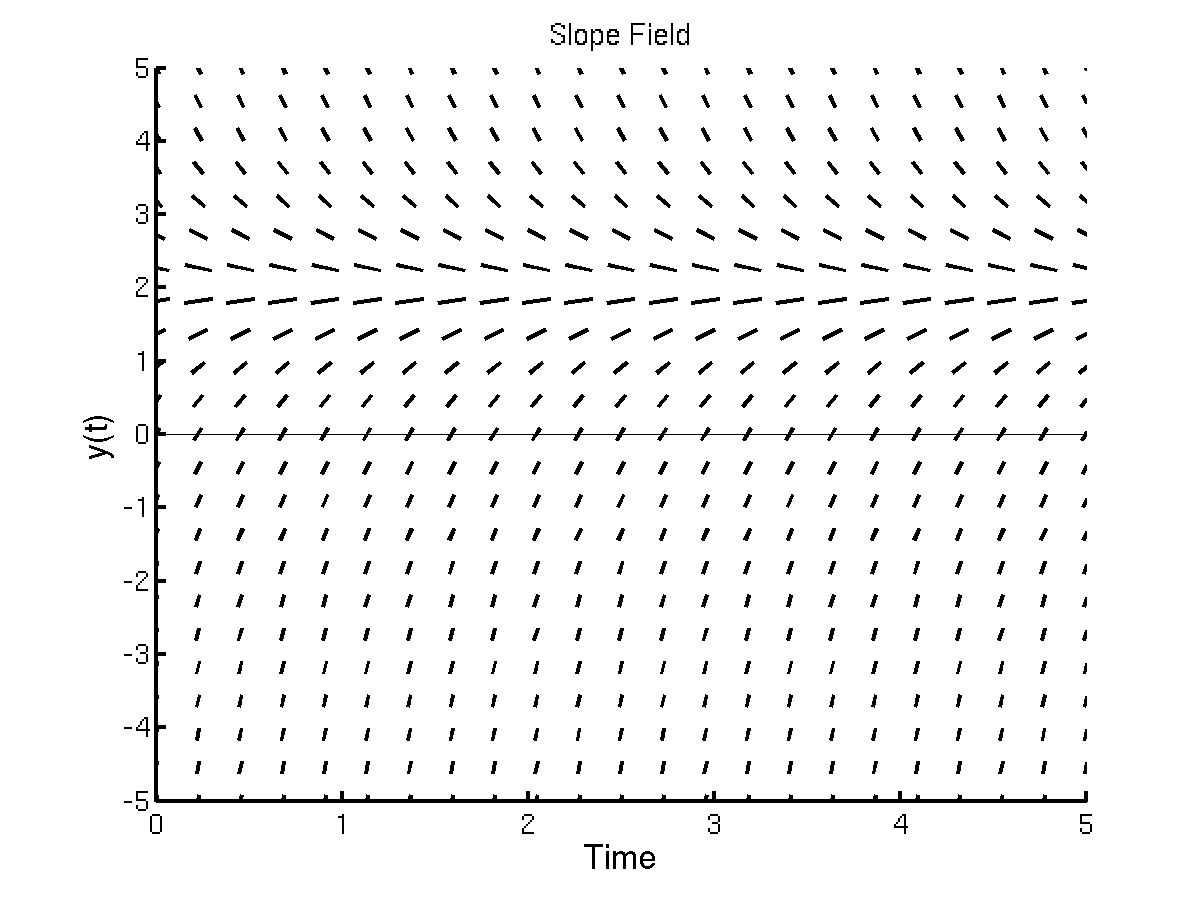
\includegraphics[height=3.0in]{img/sfSteadyWk1}
    \item 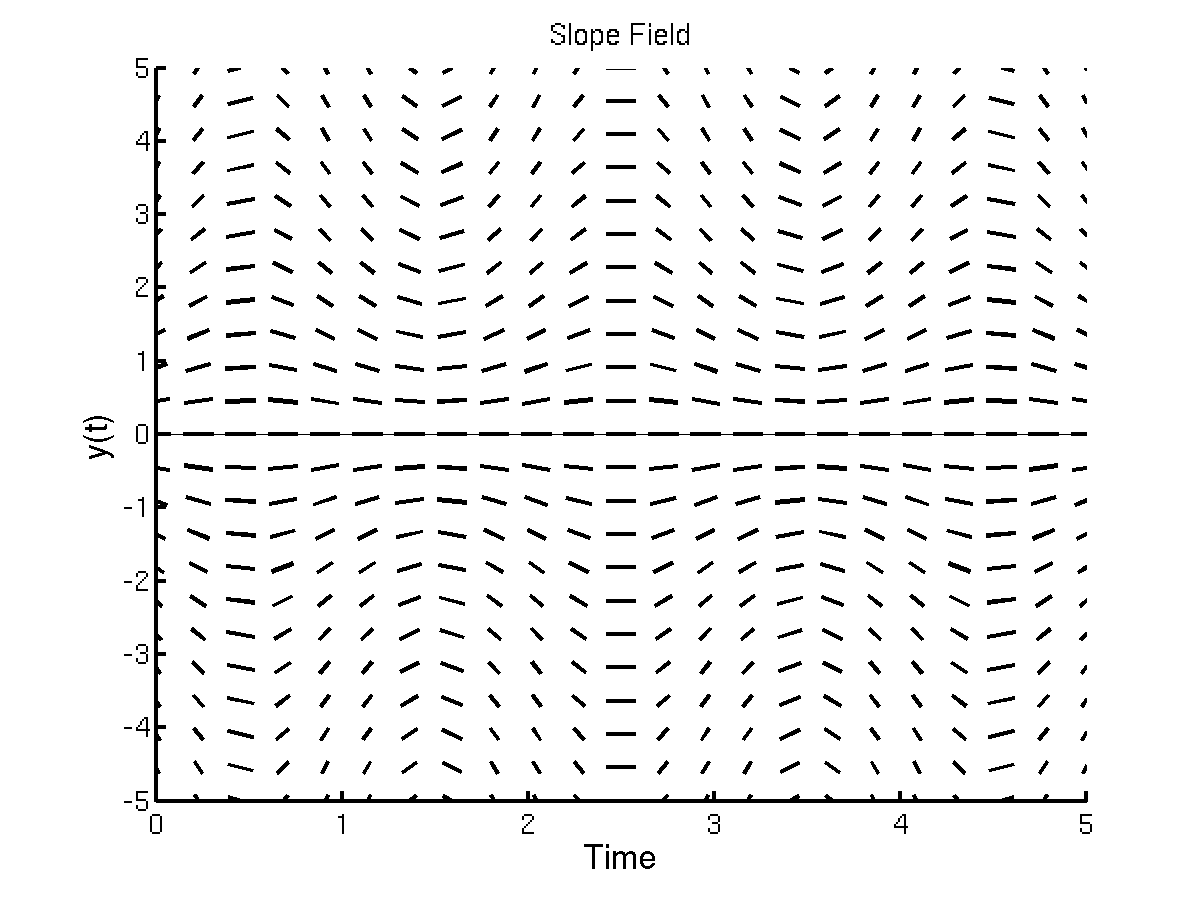
\includegraphics[height=3.0in]{img/sfOscillateWk1}

      \clearpage

    \item 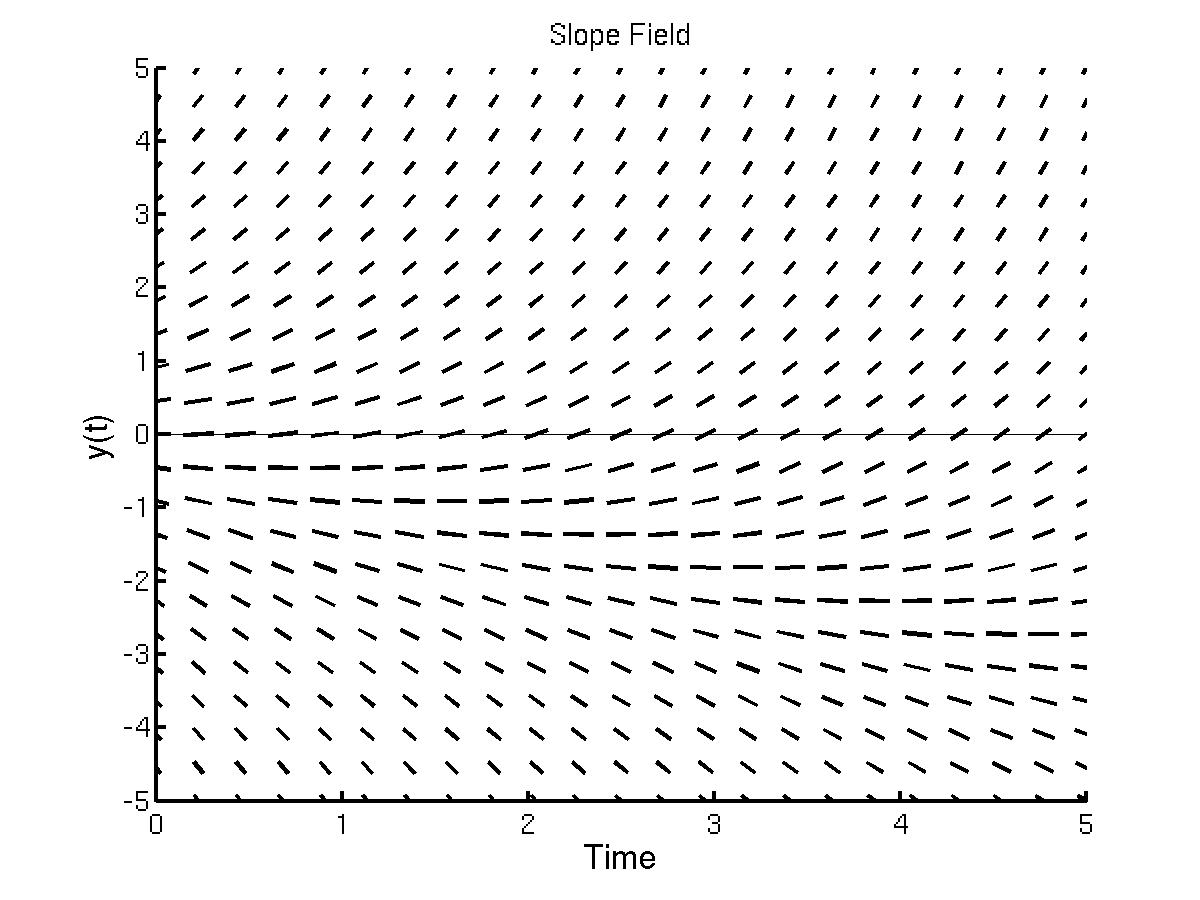
\includegraphics[height=4.0in]{img/sfLinearWk1}
    \item 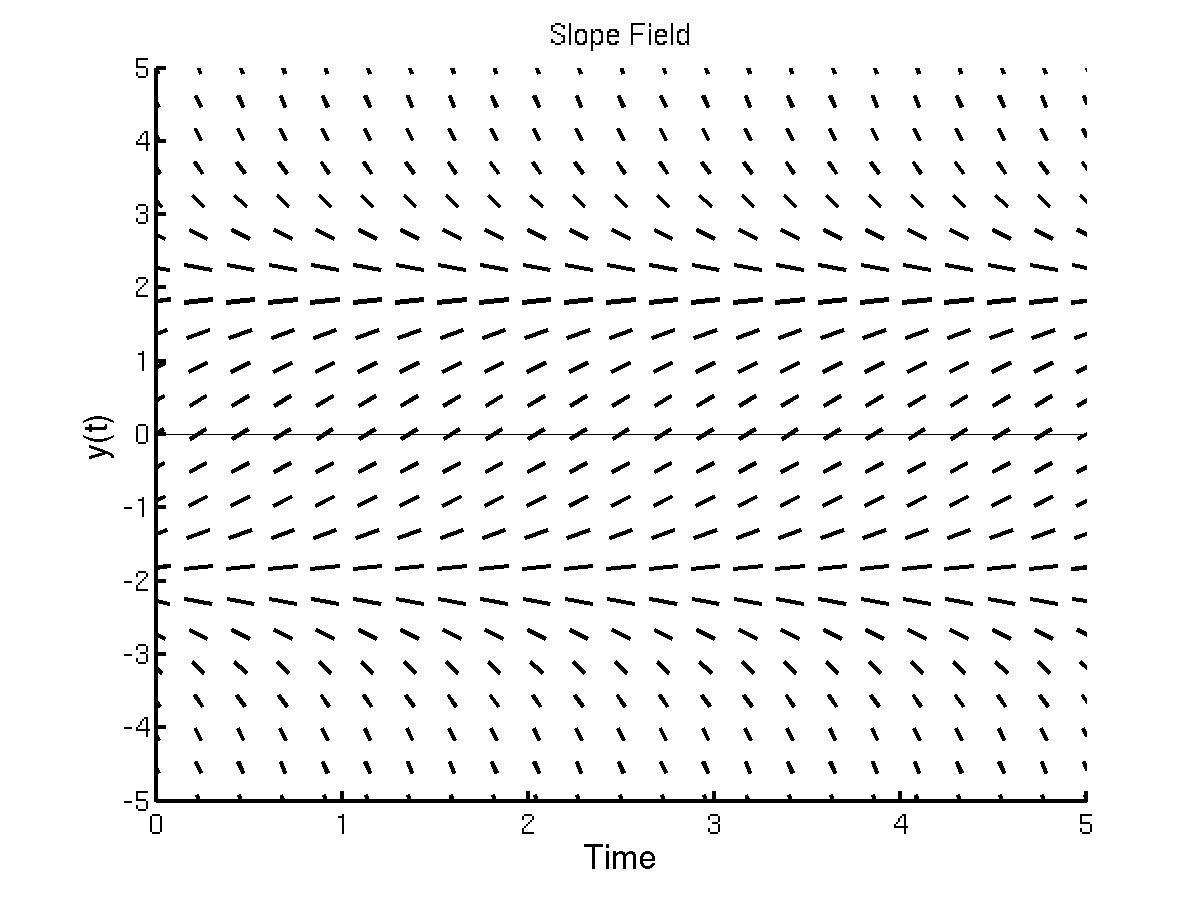
\includegraphics[height=4.0in]{img/sfStabilityWk1}

  \end{subproblem}

\clearpage

\item Make a sketch of the slope field for the equation
  \begin{eqnarray*}
    y' & = & -y^2 + 3y - 2.
  \end{eqnarray*}

  \iftoggle{solutions}{%
    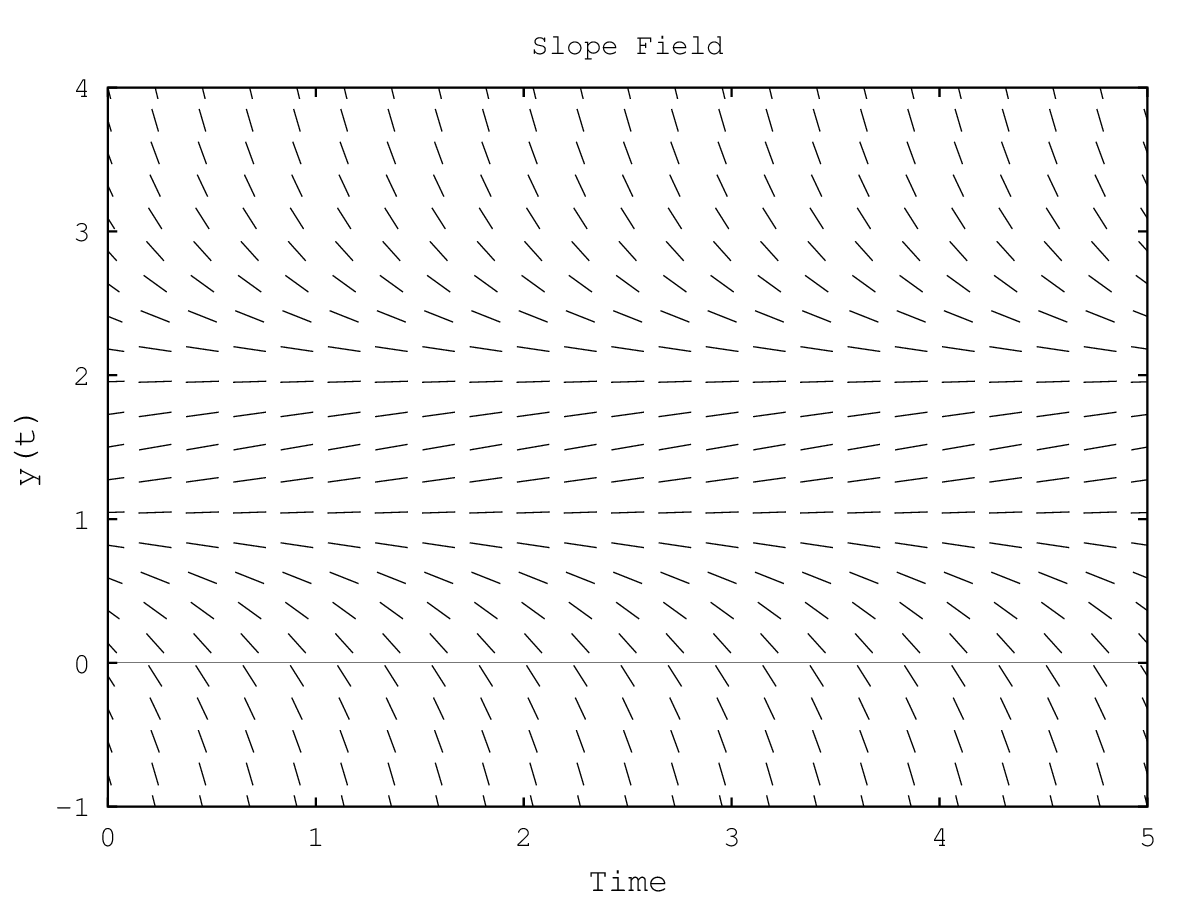
\includegraphics[height=3.0in]{img/sfDrawOwnSolutionWk1}
  }{%
    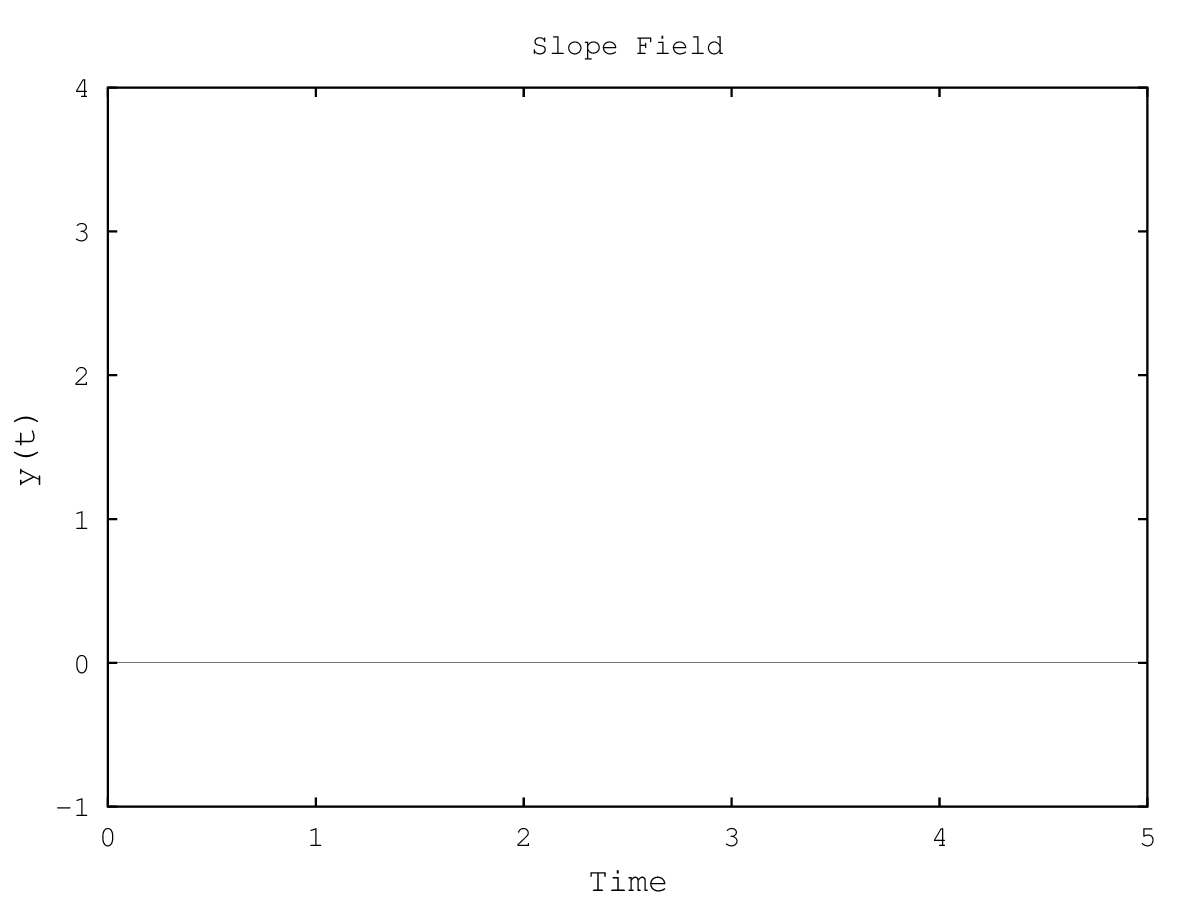
\includegraphics[height=3.0in]{img/sfDrawOwnWk1}
  }

\end{problem}


\actTitle{The Chain Rule}
\begin{problem}
\item Suppose that the function $y(t)$ satisfies the relationship
  $3t+C=\ln(y(t))$ where $C$ is a constant. Solve the equation for
  $y(t)$.

      \iftoggle{solutions}{%

        \begin{eqnarray*}
          e^{3t+C} & = & y
        \end{eqnarray*}

      }

    \vfill

  \item The function $y(t)$ depends on $t$. Use the chain rule to find
    the derivative of the expression $\ln(y(t))$.

      \iftoggle{solutions}{%

        \begin{eqnarray*}
          \frac{1}{y(t)} y'(t)
        \end{eqnarray*}
        
      }

    \vfill

  \item Show that the relationship $3t+C=\ln(y(t))$ can also be
    expressed as $y'=3y$.

      \iftoggle{solutions}{%

        \begin{eqnarray*}
          \frac{d}{dt} \lp 3t + C \rp & = & \frac{d}{dt} \ln(y(t)), \\
          3 & = & \frac{1}{y(t)} y'(t), \\
          y'(t) & = & 3 y(t).
        \end{eqnarray*}
        
      }

    \vfill

    \clearpage


  \item Show that for any constant $k$ the function
    \begin{eqnarray*}
      y(t) & = & k e^{5t}
    \end{eqnarray*}
    is a solution to the differential equation 
    \begin{eqnarray*}
      y' & = & 5y.
    \end{eqnarray*}

      \iftoggle{solutions}{%

        \begin{eqnarray*}
          y'(t) & = & 5k e^{5t}, \\
          5y(t) & = & 5k e^{5t}.
        \end{eqnarray*}
        The left hand side is equal to the right hand side.

      }

    \vfill


  \item Determine the general solution to the differential equation,
    \begin{eqnarray*}
      y'(t) & = & -7 y.
    \end{eqnarray*}

      \iftoggle{solutions}{%

        \begin{eqnarray*}
          y(t) & = & k e^{-7t},
        \end{eqnarray*}
        where $k$ is a constant.
        
      }



    \vfill

\end{problem}

% LocalWords:  dy dt
